
%(BEGIN_QUESTION)
% Copyright 2015, Tony R. Kuphaldt, released under the Creative Commons Attribution License (v 1.0)
% This means you may do almost anything with this work of mine, so long as you give me proper credit

\noindent

\vskip 5pt


\textbf{Arbidsoppdrag -- introdusjon}

Målet med oppgaven er å lære hvordan vi justerer en pressostat

$$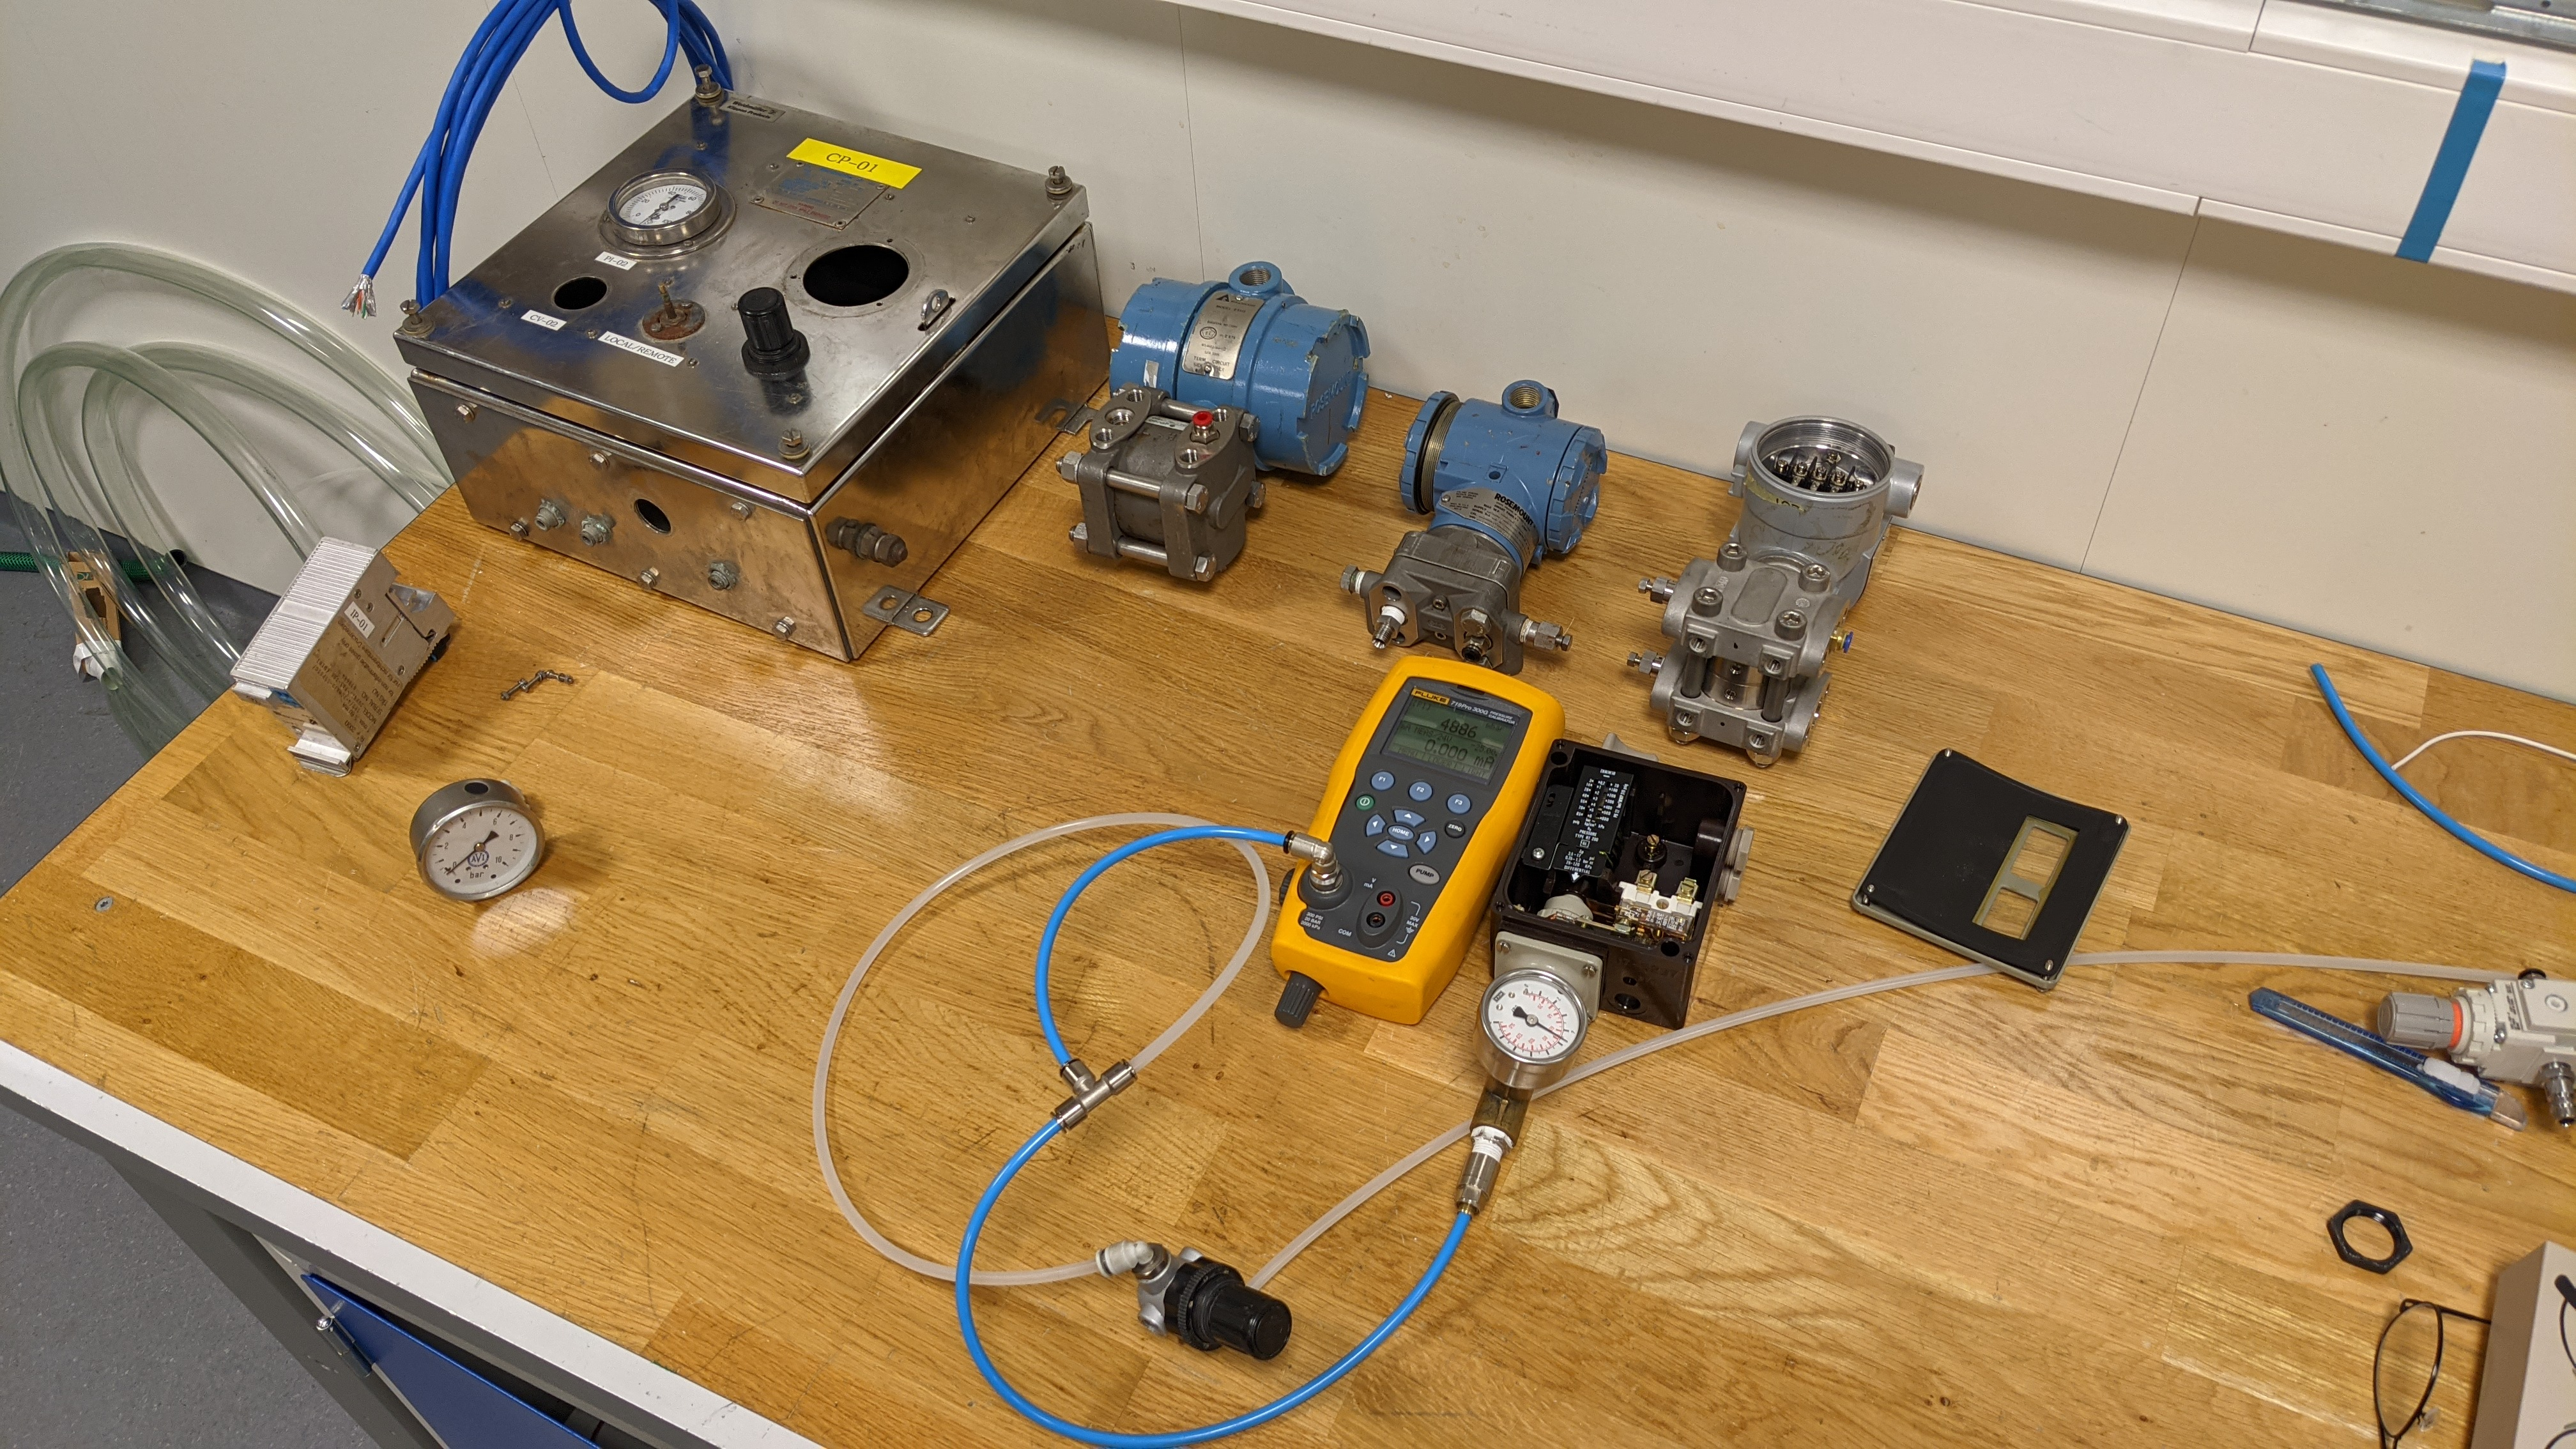
\includegraphics[width=13cm]{i04842x01.jpg}$$\\


\textbf{Arbidsoppdrag -- teorioppgaver}

\begin{enumerate}
	\item Les vedlagt bruksanvisning for å sette dere inn i virkemåten til utstyret.
\end{enumerate}
\textbf{Arbidsoppdrag -- planlegging}

Utstyr:
\begin{itemize}[noitemsep]
	\item Trykkbryter danfoss
	\item trykkregulator og manometer
	\item multimeter
\end{itemize}

\textbf{Arbidsoppdrag -- gjennomføring}

Oppgaver\begin{enumerate}
	\item Utført en As found kalibrering 
	\item Vi ønsker å bruke pressostaten til å styre tanktrykket i et hydroforanlegg. Maksimalt pumpetrykk skal være 6 barg og laveste trykke 5 barg. 
	\item Bruk instruksjons arket til å justere pressostaten.
	\item Utfør en As left kalibrering 
\end{enumerate}
\textbf{Arbidsoppdrag -- dokumentasjon}

\begin{enumerate}
	\item Beskriv hvordan du planla, gjennomførte og dokumentere jobben. Forklar hvordan en slik pressostat kan nyttes til en pumpe eller kompressor. Forklar eventuelle avvik dere måtte observere under forsøket. 
\end{enumerate}


\textbf{Arbidsoppdrag -- introdusjon}

Målet med oppgaven er å lære hvordan vi justerer en pressostat



\textbf{Arbidsoppdrag -- teorioppgaver}

\begin{enumerate}
	\item Les vedlagt bruksanvisning for å sette dere inn i virkemåten til utstyret.
\end{enumerate}
\textbf{Arbidsoppdrag -- planlegging}

Utstyr:
\begin{itemize}[noitemsep]
	\item Trykkbryter danfoss
	\item trykkregulator og manometer
	\item multimeter
\end{itemize}

\textbf{Arbidsoppdrag -- gjennomføring}

Oppgaver\begin{enumerate}
	\item Utført en As found kalibrering 
	\item Vi ønsker å bruke pressostaten til å styre tanktrykket i et hydroforanlegg. Maksimalt pumpetrykk skal være 6 barg og laveste trykke 5 barg. 
	\item Bruk instruksjons arket til å justere pressostaten.
	\item Utfør en As left kalibrering 
\end{enumerate}
\textbf{Arbidsoppdrag -- dokumentasjon}

\begin{enumerate}
	\item Beskriv hvordan du planla, gjennomførte og dokumentere jobben. Forklar hvordan en slik pressostat kan nyttes til en pumpe eller kompressor. Forklar eventuelle avvik dere måtte observere under forsøket. 
\end{enumerate}




\textbf{Arbidsoppdrag -- introdusjon}

\textbf{Kalibrering og justering range for en smart transmitter}
Målet med oppgaven er å lære hvordan vi justerer en transmitter for trykk.



\textbf{Arbidsoppdrag -- teorioppgaver}

\begin{enumerate}
	\item Sett deg inn i manualen til aktuell DP-celle
\end{enumerate}
\textbf{Arbidsoppdrag -- planlegging}

Utstyr:
\begin{itemize}[noitemsep]
	\item Trykktransmitter med HART kommunikasjon 
	\item Utstyr for å trykksette og å måle trykk 
	\item HART-communicator 
	\item +24VDC strømforsyning 
\end{itemize}

\textbf{Arbidsoppdrag -- gjennomføring}

Oppgaver\begin{enumerate}
	\item		Utført en As found kalibrering 
	\item		Bruk HART-communitatoren til å justere transmitteren slik at den gir 4 mA ved 1 barg og 20mA ved 6 barg 
	\item		Utfør en As left kalibrering 
\end{enumerate}
\textbf{Arbidsoppdrag -- dokumentasjon}

\begin{enumerate}
	\item Beskriv hvordan du planla, gjennomførte og dokumentere jobben. Forklar eventuelle avvik dere måtte observere under oppdraget. 
\end{enumerate}



\textbf{Arbidsoppdrag -- introdusjon}

Målet med oppgaven er å lære hvordan vi justerer en transmitter for trykk.



\textbf{Arbidsoppdrag -- teorioppgaver}

\begin{enumerate}
	\item Sett deg inn i manualen til aktuell DP-celle
\end{enumerate}
\textbf{Arbidsoppdrag -- planlegging}

Utstyr:
\begin{itemize}[noitemsep]
	\item analog DP-celle 
	\item Utstyr for å trykksette og å måle trykk 
	\item +24VDC strøforsyning 
	\item multimeter/sløyfekalibrator
\end{itemize}

\textbf{Arbidsoppdrag -- gjennomføring}

Oppgaver\begin{enumerate}
	\item Utfør en As found kalibrering. Tegn opp en skisse av oppkoblingen med alle komponentene med.
	\item Måleområdets laveste trykk inn velges til 0 barg og høyeste trykk velges til 7 barg.
	\item Området deles opp i 4-5 punkter og kalibreringssertefikat fylles ut med stigende og fallende verdier for transmitteren før dere justerer på den. Det er viktig å justere riktig veg når dere skal lese av, (dvs ved stigende verdier må du ikke stille for høyt og så gå tilbake). 
	\item Etter verdiene før kalibrering er fylt ut justerer dere transmitteren slik at den viser riktig på laveste og høyeste trykk. (4 mA ved laveste og 20 mA ved høyeste verdi).
	\item Deretter fylles kolonnene for verdier etter kalibrering ut.
	\item Ut fra dataene i kalibreringssertefikatet tegner dere en graf som viser sammenhengen mellom inngangssignal og utgangssignal.
	\item Lag en kort beskrivelse av hvordan måleverdiomformeren er bygget opp og hvilket måleprinsipp som er benyttet i denne omformeren.
\end{enumerate}
\textbf{Arbidsoppdrag -- dokumentasjon}

\begin{enumerate}
	\item Beskriv hvordan du planla, gjennomførte og dokumentere jobben. Forklar eventuelle avvik dere måtte observere under oppdraget. 
\end{enumerate}









\noindent

\underbar{file i04842}
\vfil \eject
%(END_QUESTION)





%(BEGIN_ANSWER)


%(END_ANSWER)





%(BEGIN_NOTES)


%INDEX% Arbeisdoppdrag, Målesystemer, Nivå 1, Stasjon10, Kalibrering, Trykkbryter

%(END_NOTES)


